\documentclass[xcolor={dvipsnames}]{beamer}
\mode<presentation>
{
  \usetheme{Antibes}      % or try Darmstadt, Madrid, Warsaw, ...
  \usecolortheme{dolphin} % or try albatross, beaver, crane, ...
  \usefonttheme{professionalfonts}  % or try serif, structurebold, ...
  \setbeamertemplate{navigation symbols}{}
  \setbeamertemplate{caption}[numbered]
} 
\usepackage[utf8]{inputenc}
\usepackage[english]{babel}
\usepackage{multirow}
\usepackage{subfigure}
\usepackage{color}
\graphicspath{{/D:/fh/JI/latex/VE230 slides}}
\usepackage{amsmath}
\title[VE230 RC slides week 5]{VE230 RC slides Week 5}
\author{han.fang }
\date{\today}


\begin{document}
\begin{frame}
\titlepage
\end{frame}
\begin{frame}
\begin{block}{Today's contents:}
\begin{enumerate}
	\item Revisit of Boundary Value Problems
	\item Current Density and Ohm's Law
	\item Electromotive Force and Kirchhoff's Voltage Law
	\item Equation of Continuity and Kirchhoff's Current Law
\end{enumerate}
\end{block}
\end{frame}
\begin{frame}{Revisit of Boundary Value Problems}
\begin{block}{Basic form}
Laplace Equation:
$$\nabla^2 V=0.$$
And some of the other boundary conditions.
\end{block}
\pause
\begin{block}{Solution: (three situations and three formats)}
\begin{itemize}
	\item $X=Ae^{-k_1x}+Be^{k_1x},\quad Y=Ce^{-k_2x}+De^{k_2x}$
	\item $X=A\sin(k_1x)+B\cos(k_1x),\quad Y=C\sin(k_2x)+D\cos(k_2x)$
	\item $X=a+bx,\quad Y=c+dx$
\end{itemize}
\end{block}
\end{frame}
\begin{frame}
\begin{block}{How to solve???}
\begin{enumerate}
	\item First, write out the expansion of the Laplace Equation, i.e.,
	$$\nabla^2 V=\frac{\partial^2 V}{\partial x^2}+\frac{\partial^2 V}{\partial y^2}+\frac{\partial^2 V}{\partial z^2}=0$$
	\item According to the boundary conditions given, judge whether $V$ is independent of the variable. 
	\item If there is only one variable left, then the solution is the third format, i.e., $X=a+bx,\quad Y=c+dx$. Then use the boundary conditions to find the parameter of the solution.
	\item If there is more than one variable involved, then tried the first format and second format to find if they can satisfy the boundary conditions. If one of the formats can be found that satisfies the boundary conditions, then stop, because of the uniqueness theorem.
\end{enumerate}
\end{block}
\end{frame}
\begin{frame}{Example}
\begin{figure}
	\centering
	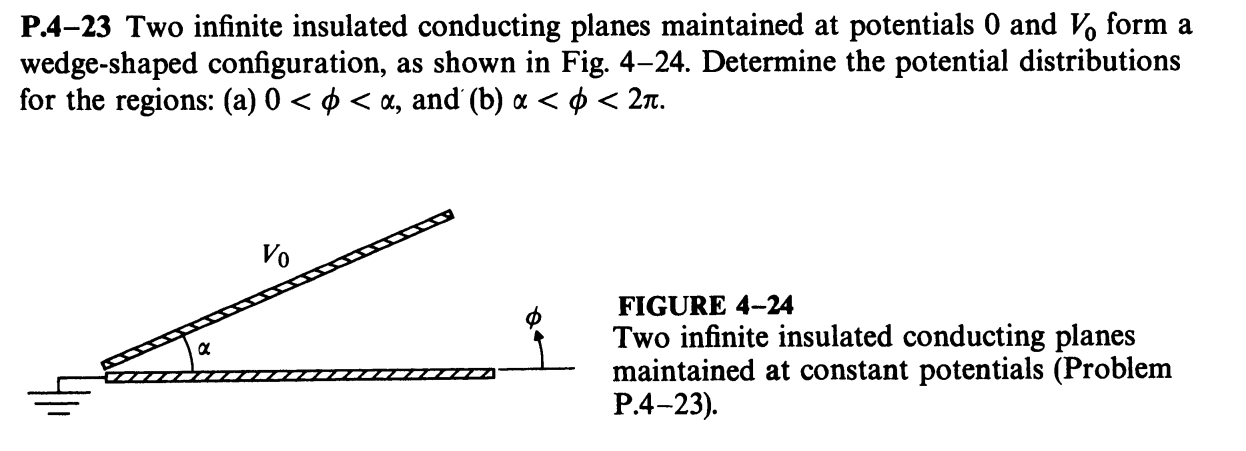
\includegraphics[width=0.8\linewidth]{5_16.png}
\end{figure}
\pause
\begin{figure}
	\centering
	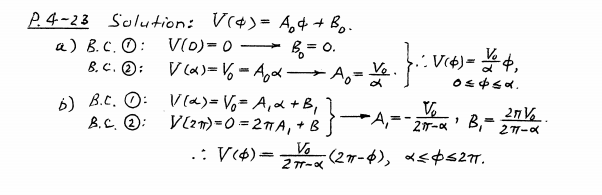
\includegraphics[width=0.8\linewidth]{5_17.png}
\end{figure}
\end{frame}
\begin{frame}
Types of electric currents caused by the motion of free charges:
\begin{enumerate}
  \item \textbf{conduction currents}: drift motion of conduction electrons and/or holes in conductors/semiconductors.
  \item electrolytic currents: migration of positive and negative ions.
  \item convenction currents: motion of electrons and/or ions in a vacuum.
\end{enumerate}
\end{frame}
\begin{frame}{Current Density and Ohm's Law}
$$I = \int_S \vec{J}\cdot d\vec{s}\quad (A)$$

where $\vec{J}$ is the volume current density or current density, defined by 

$$\vec{J} = Nq\vec{u}\quad (A/m^2)$$,

where $N$ is the number of charge carriers per unit volume, each of charges $q$ moves with a velocity $\vec{u}$.

Since $Nq$ is the free charge per unit volume, by $\rho = Nq$, we have:
$$
\vec{J} = \rho \vec{u}\quad (A/m^2)
$$
\end{frame}
\begin{frame}{Current Density and Ohm's Law}
For conduction currents,

$$
\vec{J} = \sigma \vec{E} \quad (A/m^2)
$$

where $\sigma = \rho_e\mu_e$ is conductivity, a macroscopic constitutive parameter of the medium. $\rho_e = -Ne$ is the charge density of the drifting electrons and is negative. $\vec{u} = -\mu_e \vec{E} \quad(m/s)$ where $\mu_e$ is the electron mobility measured in $(m^2/V\cdot s)$.

Materials where $
\vec{J} = \sigma \vec{E} \quad (A/m^2)
$ holds are called ohmic media. The form can be referred as the point form of Ohm's law.

\textbf{Derivation of voltage-current relationship of a piece of homogeneous material by the point form of Ohm's law.}
\end{frame}
\begin{frame}{Current Density and Ohm's Law}
\begin{figure}[H]
  \centering
  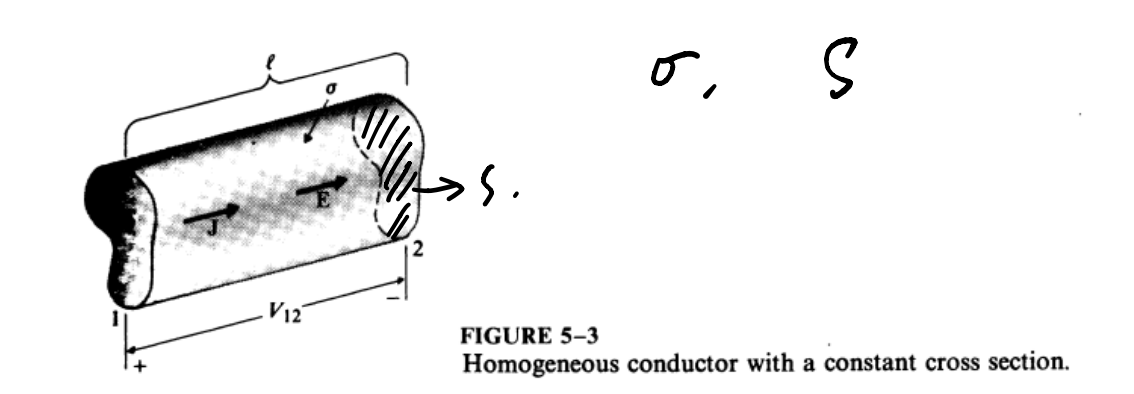
\includegraphics[width=0.7\linewidth]{5_15.png}
\end{figure}
Thus, the resistance is defined as
$$
R = \frac{l}{\sigma S} \quad (\Omega)
$$

where $l$ is the length of the homogeneous conductor, $S$ is the area of the uniform cross section.
\end{frame}
\begin{frame}{Current Density and Ohm's Law}
The conductance $G$ (reciprocal of resistance), is defined by 

$$
G=\frac{1}{R} = \sigma \frac{S}{l}\quad (S)
$$

\begin{enumerate}
  \item Resistance in series: $$R_{sr} = R_1 + R_2$$
  \item Resistance in parallel: $$\frac{1}{R_{||}} = \frac{1}{R_1} + \frac{1}{R_2}$$, or $$G_{||} = G_1+G_2$$
\end{enumerate}
\end{frame}
\begin{frame}{Electromotive Force and Kirchhoff's Voltage Law}
A steady current cannot be maintained in the same direction in a closed circuit by an electrostatic field, which is:

$$
\oint_C \frac{1}{\sigma}\vec{J}\cdot d\vec{l} = 0
$$

Kirchhoff's voltage law: around a closed path in an electric circuit, the algebraic sum of the emf's (voltage rises) is equal to the algebraic sum of the voltage drops across the resistance, which is:
$$
\sum_j V_j = \sum_k R_k I_k\quad (V)
$$
\end{frame}
\begin{frame}{Equation of Continuity and Kirchhoff's Current Law}
Equation of continuity:

$$
\nabla\cdot\vec{J} = -\frac{\partial \rho}{\partial t} \quad (A/m^3)
$$,

where $\rho$ is the volume charge density. 

For steady currents, as $\partial \rho/\partial t= 0$, $\nabla\cdot \vec{J}=0$. By integral, we have Kirchhoff's current law, stating that the algebraic sum of all the currents flowing out of a junction in an electric circuit is zero: 
$$
\sum_j I_j = 0
$$

\end{frame}
\begin{frame}{Equation of Continuity and Kirchhoff's Current Law}
For a simple medium conductor, the volume charge density $\rho$ can be expressed as:

$$
\rho = \rho_0 e^{-(\rho/\epsilon)t}\quad (C/m^3)
$$

where $\rho_0$ is the initial charge density at $t=0$. The equation implies that the charge density at a given location will decrease with time exponentially. 


Relaxation time: an initial charge density $\rho_0$ will decay to $1/e$ or $36.8\%$ of its original value:
$$
\tau = \frac{\epsilon}{\sigma}\quad(s)
$$
\end{frame}
\begin{frame}{Assignment Part}
\begin{figure}[H]
	\centering
	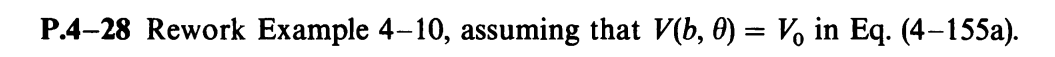
\includegraphics[width=0.9\linewidth]{5_0.png}
\end{figure}
\begin{figure}[H]
	\centering
	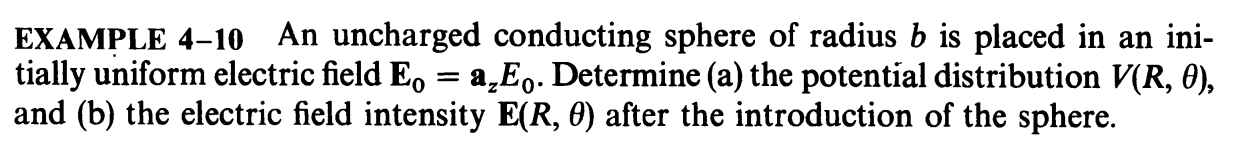
\includegraphics[width=0.9\linewidth]{5_1.png}
\end{figure}
\end{frame}
\begin{frame}
\begin{figure}[H]
	\centering
	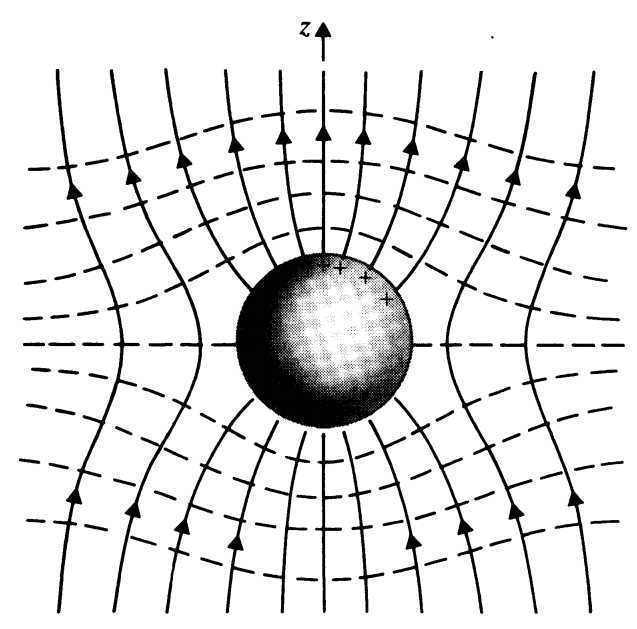
\includegraphics[width=0.8\linewidth]{5_5.png}
\end{figure}
\end{frame}
\begin{frame}
\begin{figure}[H]
	\centering
	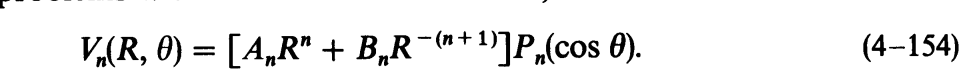
\includegraphics[width=0.9\linewidth]{5_6.png}
\end{figure}
\begin{figure}[H]
	\centering
	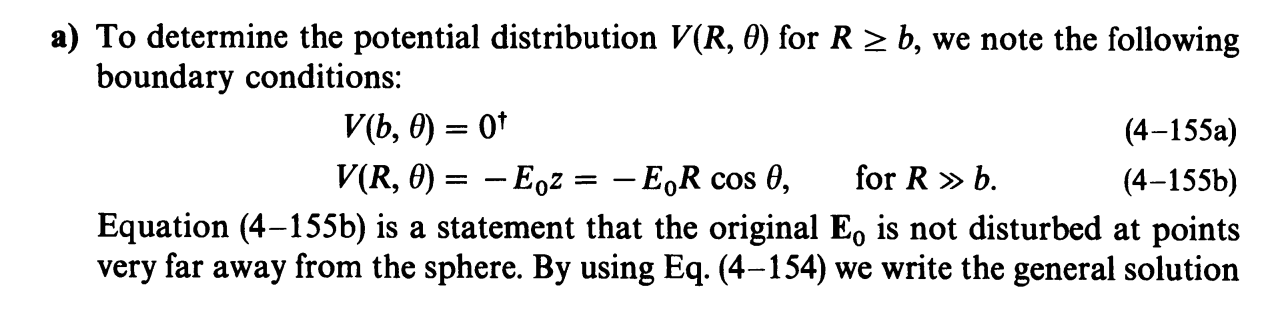
\includegraphics[width=0.9\linewidth]{5_3.png}
\end{figure}
\begin{figure}[H]
	\centering
	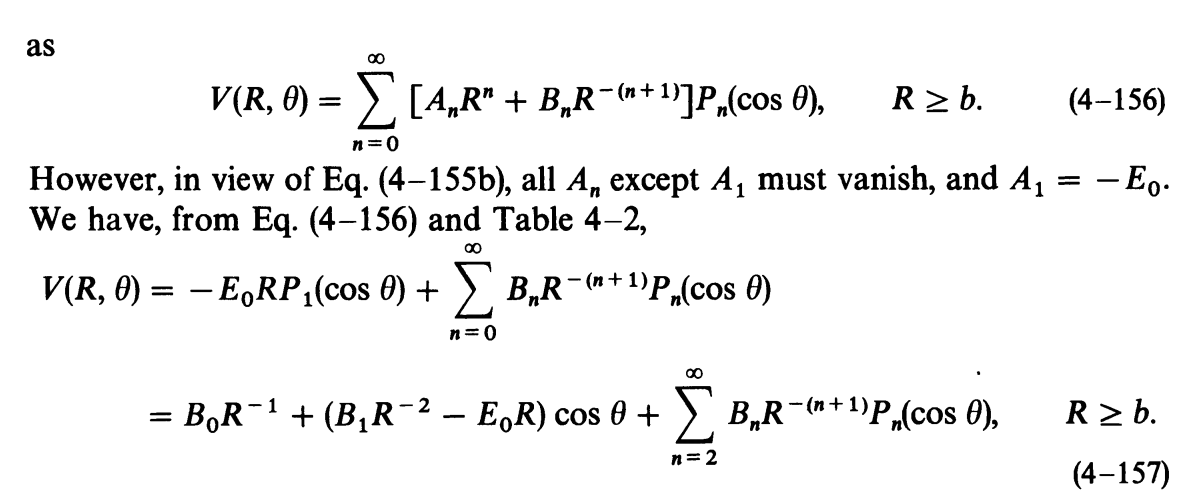
\includegraphics[width=0.9\linewidth]{5_4.png}
\end{figure}
\end{frame}
\begin{frame}
\begin{figure}[H]
	\centering
	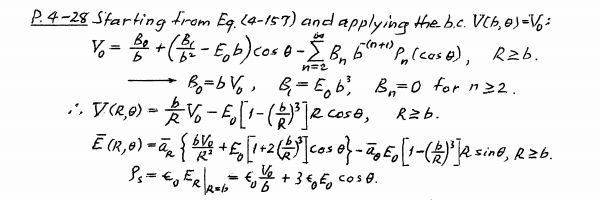
\includegraphics[width=0.9\linewidth]{5_2.png}
\end{figure}
\end{frame}
\begin{frame}
\begin{figure}[H]
	\centering
	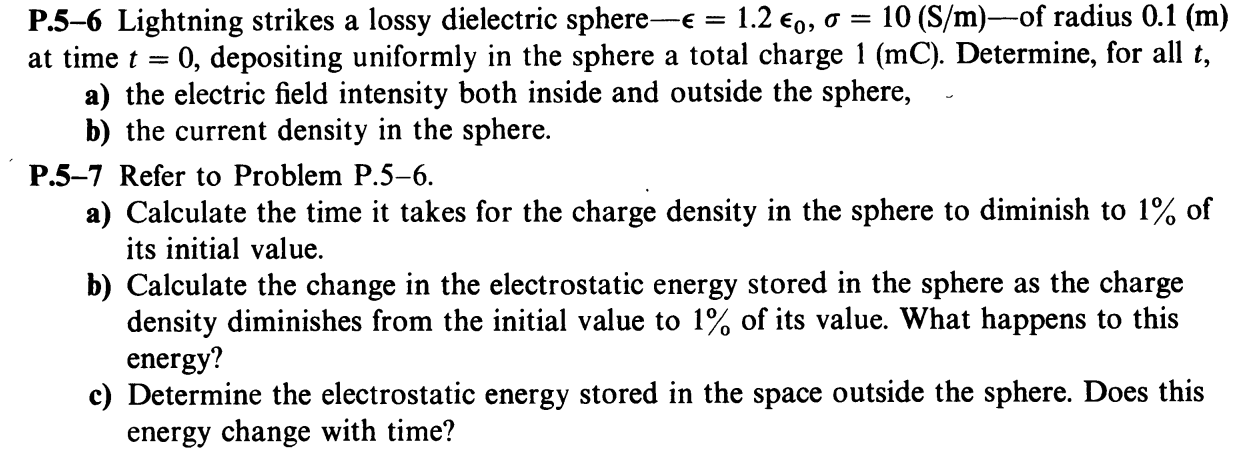
\includegraphics[width=0.9\linewidth]{5_7.png}
\end{figure}
\pause
\begin{figure}[H]
	\centering
	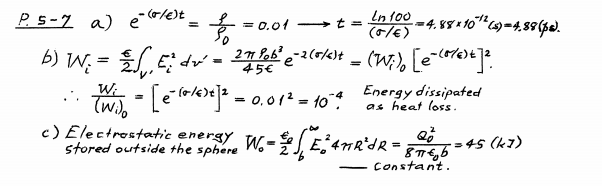
\includegraphics[width=0.9\linewidth]{5_8.png}
\end{figure}
\end{frame}
\begin{frame}
\begin{figure}[H]
	\centering
	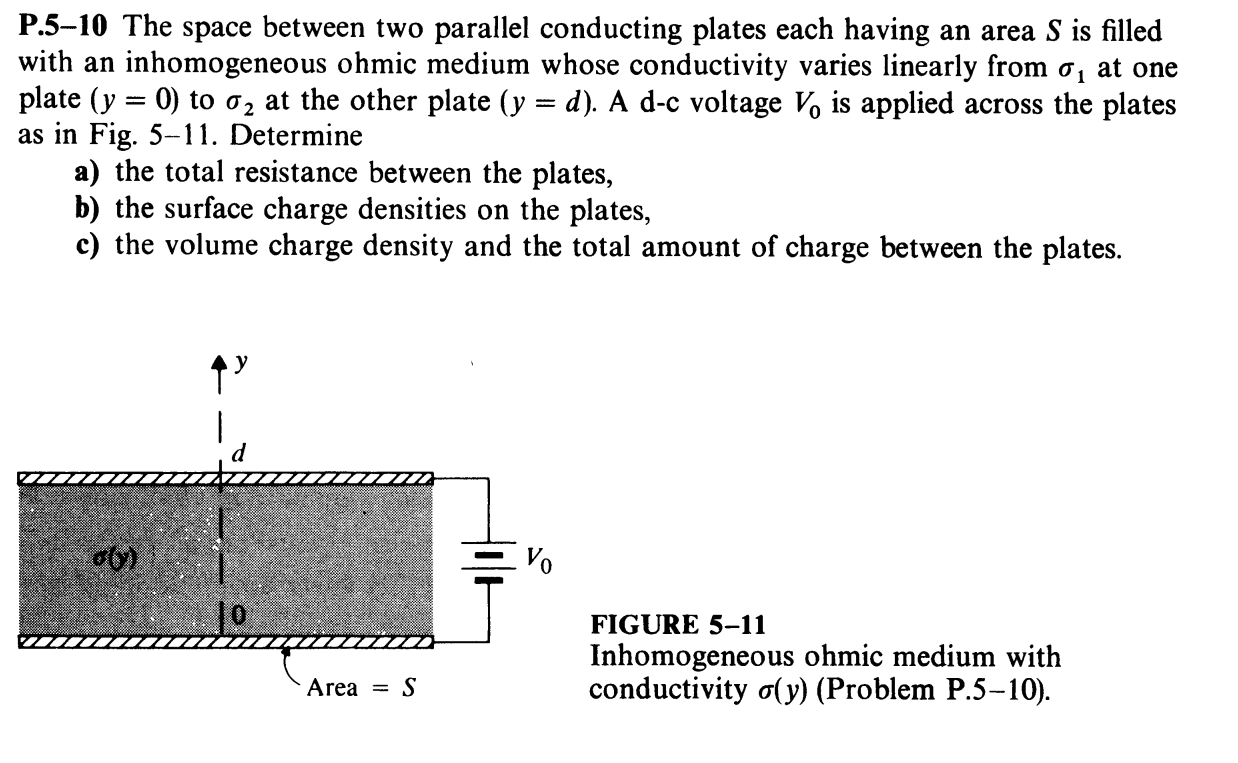
\includegraphics[width=0.9\linewidth]{5_9.png}
\end{figure}

\end{frame}
\begin{frame}
\begin{figure}[H]
	\centering
	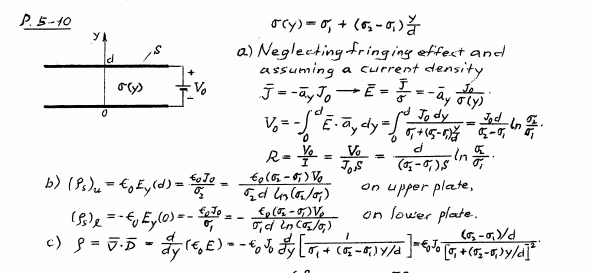
\includegraphics[width=0.9\linewidth]{5_10.png}
\end{figure}

\end{frame}
\begin{frame}
\begin{figure}[H]
	\centering
	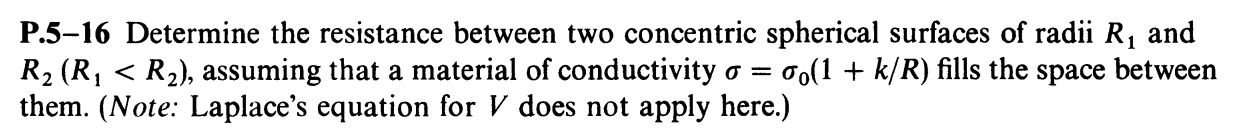
\includegraphics[width=0.9\linewidth]{5_11.png}
\end{figure}
\pause
\begin{figure}[H]
	\centering
	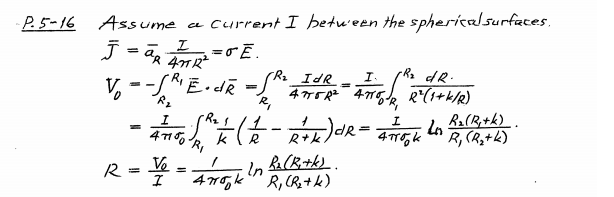
\includegraphics[width=0.9\linewidth]{5_12.png}
\end{figure}
\end{frame}
\begin{frame}
\begin{figure}[H]
	\centering
	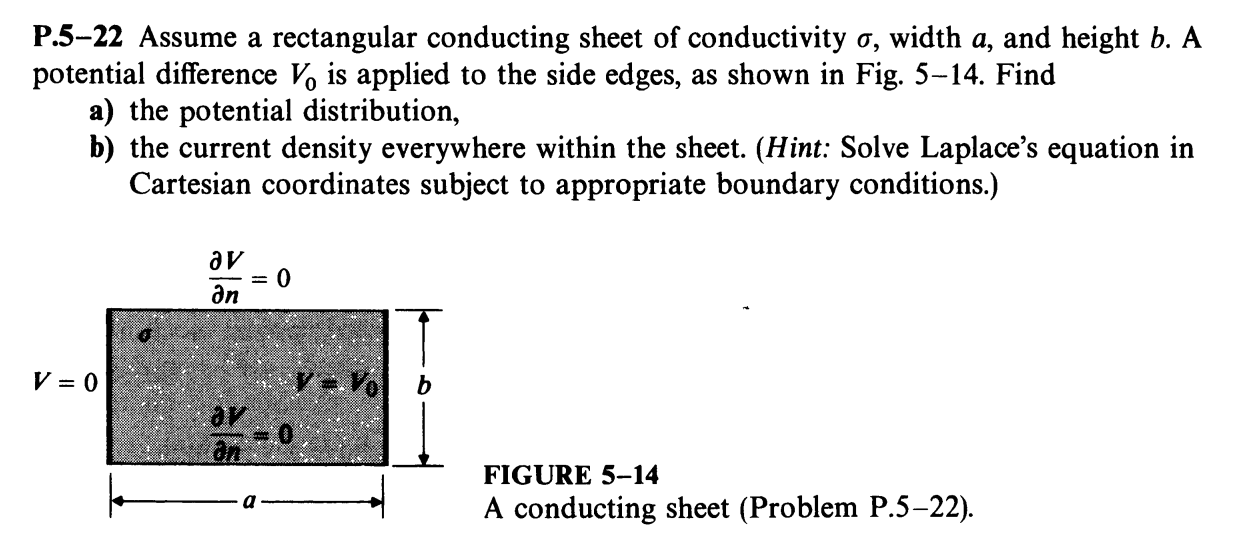
\includegraphics[width=0.9\linewidth]{5_13.png}
\end{figure}
\pause
\begin{figure}[H]
	\centering
	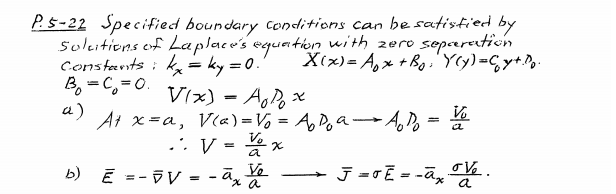
\includegraphics[width=0.9\linewidth]{5_14.png}
\end{figure}
\end{frame}
\end{document}